\section{Control loop}
% Control Loop (differences between the two, from where they start to where they close, freuqency for the various elements)

\begin{frame}{Control loop}

    \begin{columns}[c, onlytextwidth]

        \begin{column}{0.6\textwidth}

            \begin{figure}
                \centering
                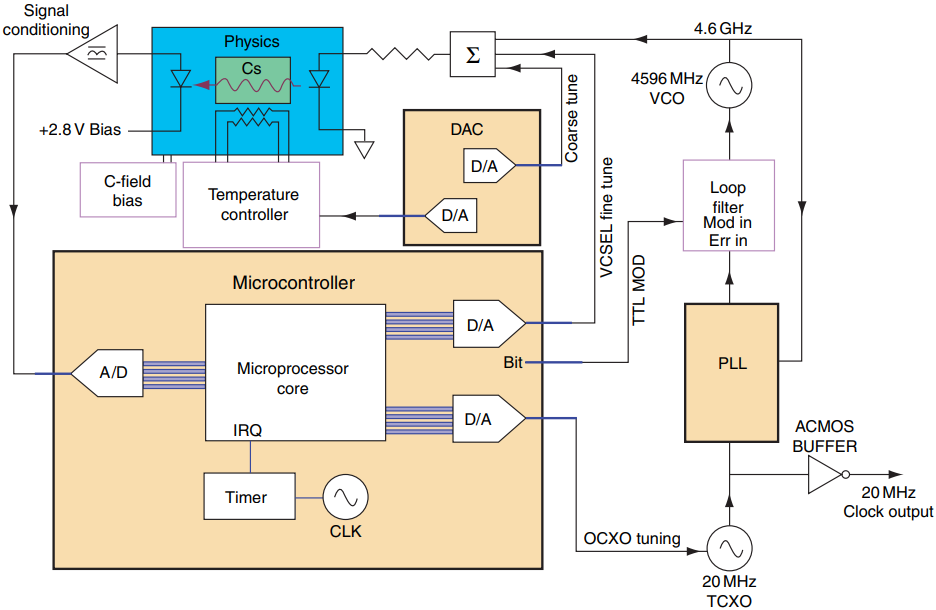
\includegraphics[width=0.9\textwidth]{img/Control-loop}
                \caption{Control loop block diagram.}
            \end{figure}

        \end{column}

        \begin{column}{0.4\textwidth}

            Close-loop control approach.
            Usually multiple PI controllers are used to operate a series of servo loops.

            \vspace{10pt}

            Indispensable targets:

            \begin{itemize}
                \item Laser temperature
                \item Cell temperature
                \item Laser frequency
                \item LO frequency
            \end{itemize}

        \end{column}

    \end{columns}

\end{frame}



\begin{frame}{Electronics}

    Here are some possible problematic areas:

    \begin{itemize}
        \item Stability in the voltage and current provided to VCO and VCSEL (highly sensitive components)
        \item Cross-talk between the various control loops
        \item Noise from the electronics
        \item Power consumption
    \end{itemize}

\end{frame}